\section{Experimental Setup}\label{sec:experimentalSetup}

Our goal is to build an in-depth understanding about
the performance of the \mas for detecting malware. \review{To this
end, we replicate previous studies using a dataset of repackaged apps that is an order of magnitude
larger than the datasets used before~\cite{DBLP:conf/wcre/BaoLL18,DBLP:journals/jss/CostaMMSSBNR22}.} Accordingly,
we investigate the the following research questions:

\begin{enumerate}[(RQ1)]
\item \rqa
\item \rqc
\item \rqd
% \review{\item \rqe}
\end{enumerate}

\review{In this section, we describe our study settings. First, we present the procedures we use to create our datasets (Section~\ref{sec:dataset}).  Then, we describe the data collection and data analysis procedures (Sections~\ref{sec:dataCollectionProc} and~\ref{sec:dataAnalysisProc}).}


\subsection{Malware Dataset}\label{sec:dataset}


%Our experiment aims to compute if an app pair from a given sample is a malware variant of its corresponding original app.
To investigate our research questions, we shall run our infrastructure on a representative and up-to-date dataset and estimate the \mas performance (in terms of accuracy). Our dataset shall also
be \textit{labeled}, i.e., the interest characteristic of each app, like similarity and malware family, should be known beforehand. 

\subsubsection{Procedures for Building the Dataset}

We use two repositories of repackaged Android apps (\repack and \amc) to
curate the dataset we use in our research. \repack has been curated using automatic procedures that mine repackaged apps from the Androzoo
repository~\cite{DBLP:conf/msr/AllixBKT16}, and
comprises 15,297 pairs of original and repackaged Android apps, with 2,776 unique original apps~\cite{DBLP:journals/tse/LiBK21}---
multiple repackaged versions of the same original app may coexist within \repack, \review{with a minimal, and maximum times of 1 and 176, respectively}.
However, we encountered compatibility issues with many samples, either in relation to DroidFax~\cite{DBLP:conf/icsm/CaiR17a} or the versions of the Android emulator we employed (API level 28). First, out of 2,776 original apps, DroidFax instrumented 1,915. Among these 1,915 samples, 554 apps we failed to install due Android emulator compatibility or other emulator settings. This led to the removal of 1,416 samples from the initial set of 2,776 original apps. Consequently, we selected 3,827 samples of app pairs (original/repackaged) from \repack. 

\review{Released in August 2018, the decision to use API 28 for the emulator is based on the fact that it is an intermediate version between the \repack and \amc releases. Since Android apps are forward-compatible, older apps can run on newer versions of the Android Operating System. Thus, with this decision, we aim to cover the maximum number of samples in both datasets.}

Regarding \amc, it comprises 378,546 repackaged Android apps~\cite{andromalpack}, \review{and as \repack, it has multiple repackaged version of the same orignal app, with a minimal and maximum time of 2 and 2,113.}

In contrast to \repack,
which only includes packages built until 2018, \amc includes many recent samples, some packaged as late as 2022.
Unfortunately, \amc lacks information about the original apps, leading us to employ a conservative heuristic
to identify the original versions of repackaged apps in \amc. This heuristic is based on an adapted
procedure designed to identify repackaged versions of a given app~\cite{DBLP:journals/tse/LiBK21}.
Despite our efforts, we could not identify the original version for several repackaged samples in \amc.
We also excluded samples with a package date before 2018 (so that we could avoid any overlapping with
the samples already selected from \repack), resulting in 1,190 ``app pair candidates''.
Finally, we eliminated 419 pairs that shown incompatible issues with either DroidFax (396 samples), or the versions of the Android
emulator (23 samples) used in our research (API level 28). In total, we selected 771 app pairs from \amc to curate our dataset.

%% To ensure that the pairs are indeed (original/repackaged), we also check some meta-files, like app signature~\cite{DBLP:journals/percom/MerloRSV21}. We compare the signature of original and repackaged app, and assume that, if they do not match, means that they have different developers. We also check if the repackaged app version have 
%% \textit{.dex file} create date later than the original app, to ensure that the repackaged version was developed after the original. After removing all app pair that do not meet both criteria, we were left with 1,190 app pair. As \texttt{RePack-Dataset}, we also fail to execute our study in some samples, due to same instrumentation problem or emulator compatibility. After removing 419 incompatible app pairs, we were left with 771 app pair from \texttt{AndroMalPack}. 

We combined the selected samples from \repack and \amc, resulting in a total of 4,598 app
pairs (3,827 from \repack and 771 from \amc). Subsequently, we queried the \vt repository
to identify original versions of apps labeled as malware. Samples with such labels were excluded from our dataset,
as the \mas assumes that the original version of an app is not malware (or else, the repackaged versions might
also exhibit malicious behavior). \vt, a widely recognized tool, scans software assets, including Android apps,
using over 60 antivirus engines~\cite{DBLP:journals/ese/KhanmohammadiEH19}. Thus, we excluded 616 samples from \repack and 45 samples from \amc. In the end, we are left with our \cds of \apps apps which we use in our study (3,211+726). Figure~\ref{fig:dataset} summarizes the methodology we use to extract the dataset for our study.

To bring evidence that we were able to reproduce the results of previous research, we also consider a small dataset (hereafter \sds)
used in the original studies~\cite{DBLP:conf/wcre/BaoLL18,DBLP:journals/jss/CostaMMSSBNR22}.

% I do not think the figure is helping. 

  \begin{figure}[htb]
   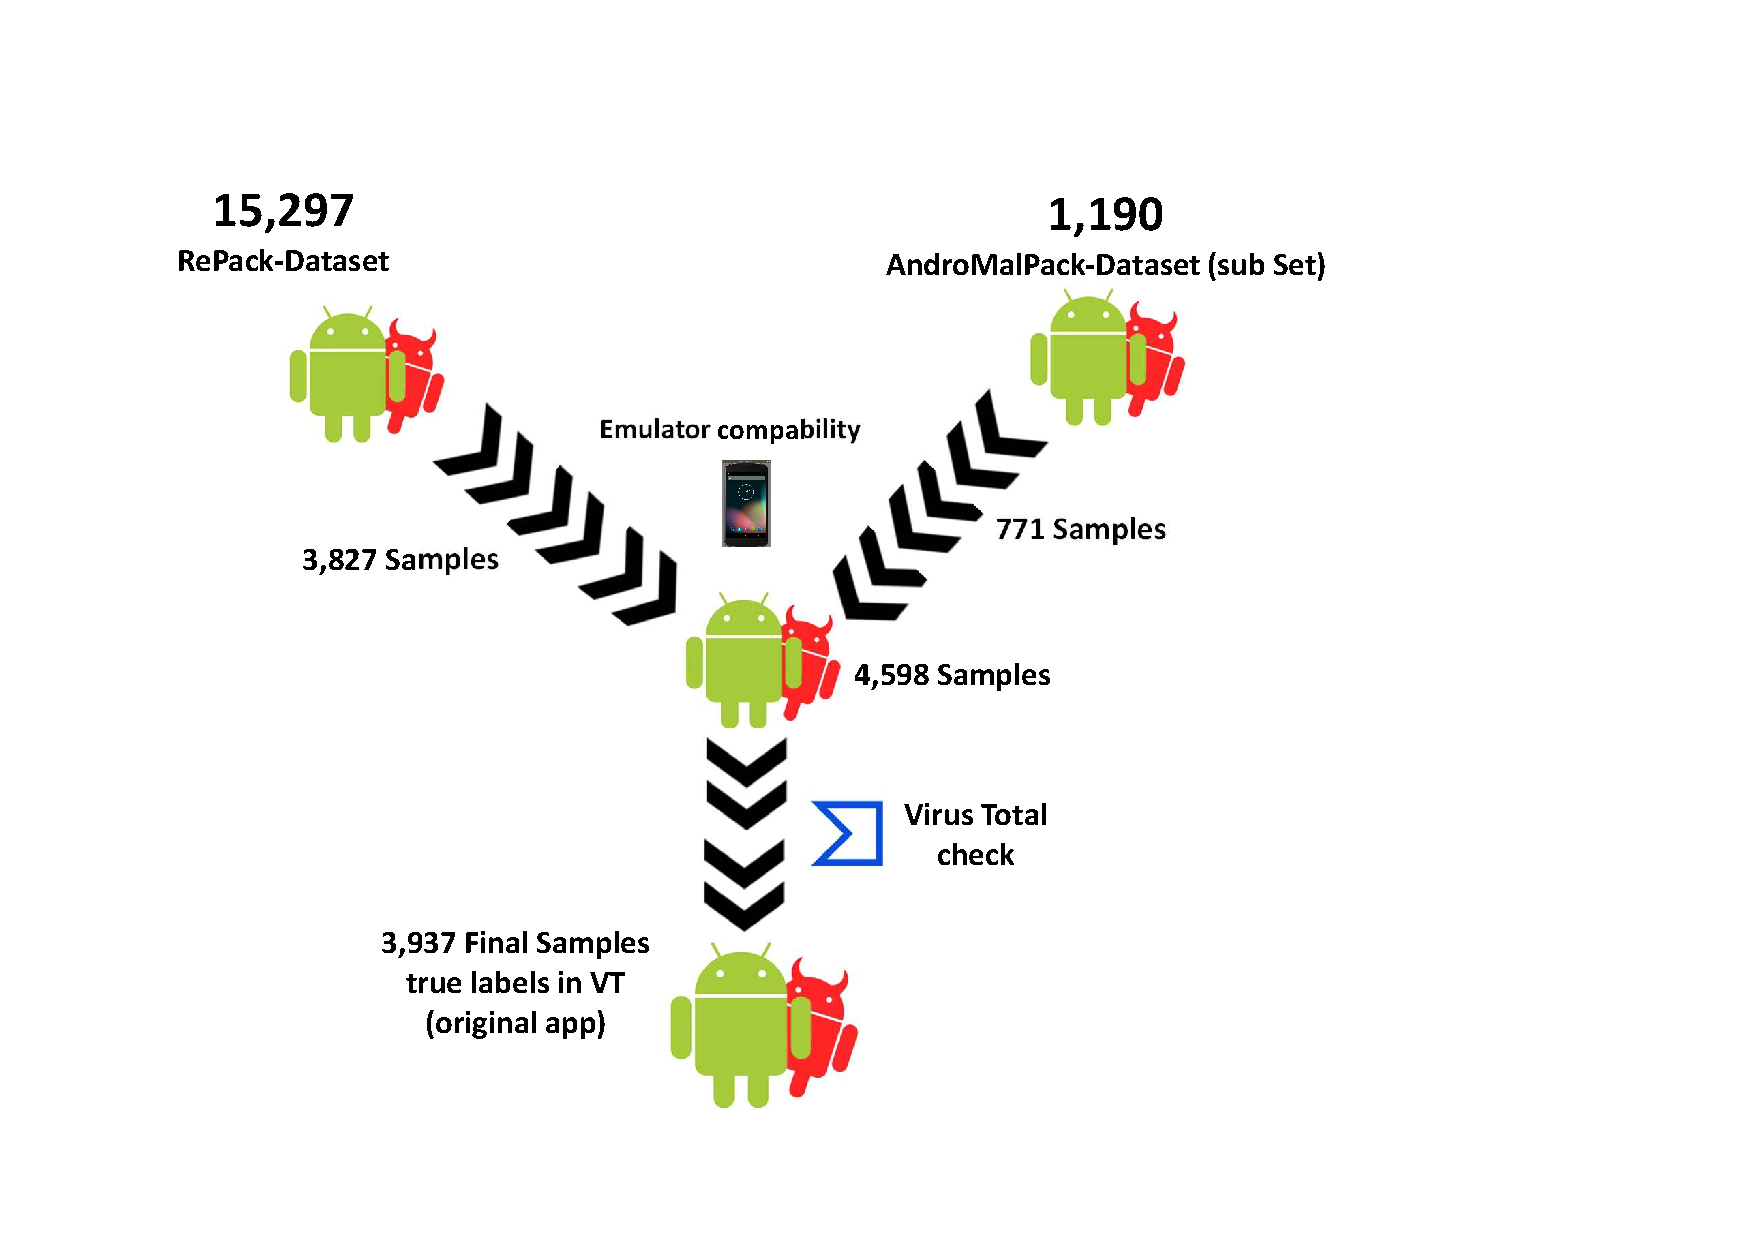
\includegraphics[width=\columnwidth]{images/dataSet_V2.pdf}
   \caption{Malware samples in \cds.}
   \label{fig:dataset}
 \end{figure}



%starting from an initial sample of 3344 repackaged pairs of apps available in AndroZoo~\cite{DBLP:conf/msr/AllixBKT16}.
%We do not use any particular criteria for selecting the initial sample.
%Nonetheless, due to compatibility issues we found---either during the instrumentation phase (using DroidFax) or during the execution
%phase using the Android emulator---we end-up with our final dataset (hereafter \cds) that contains \apps pairs of
%repackaged apps (36\% of the initial subset repackaged apps).
%\fh{At this paragraph I change the term set to Subset since 3344 is a subset of 15.000 repackage pair}

%\kn{This whole part about Virustotal needs a bit more elaboration. Ideally, including a citation explaining why we go for this additional method of classifying whether something as a malware or not. Since we already start with the app pairs, we sort of already know the malicious and benign version right? }

\subsubsection{Features of the Datasets}
 
We queried the \vt repository to find out which repackaged apps in our
dataset have been indeed labeled as a malware.
%, and we took this decision since the output of \vt can change over time~\cite{vt-label}.\fh{Here I inserted a litle discription of
% VT and inserted some reference}
%(\kn{two out of how many antiviruses are included by Virustotal}). 
According to \vt, in the \sds (102 pairs),
69 of the repackaged apps (67.64\%) have been identified as a malware by at least two
\ses. Here we only consider that a repackaged version of an app is a malware if \vt reports that at least
two \ses identify a malicious behavior within the asset. This is in accordance with previous research~\cite{vt-label,DBLP:journals/ese/KhanmohammadiEH19}. Considering the \cds, at least two security engines identified \malwares out of the \apps repackaged apps as malware (\malwaresP\%).

Classifying malware into different categories is a common practice. For instance, Android malware can be classified into categories
like riskware, trojan, adware, etc. Each category might be further specialized in several malware families, depending of its
characteristics and attack strategy---e.g., steal network info (IP, DNS, WiFi), collect phone info,
collect user contacts, send/receive SMS, and so on~\cite{DBLP:conf/iccns/RahaliLKTGM20}.
According to the
\avt~\cite{avclass2-paper}, the malware samples in the \sds come from $17$ different families---most of them from the Kuguo (49.27\%) and Dowgin (17.39\%) families.  
Our \cds, besides a large sample of repackaged apps (\apps in total),
comprises \review{116} families of malware we collected using the \avt---most
of them from the Gappusin \review{(33.78\%)} family.

We also characterize our dataset according to the similarity
between the original and repackaged versions of the apps, using the  
SimiDroid tool~\cite{DBLP:conf/trustcom/0029BK17}. SimiDroid quantifies the similarity
based on (a) the methods that are either identical or similar in both versions of the apps (original and repackaged versions),
(b) methods that only appear in the repackaged version of the apps (new methods), and (c) methods that only appear in the
original version of the apps (deleted methods).
Our \cds has an average similarity score of \review{(90.38)\%}---with the follow distribution \review{($84$ of
app pairs have a similarity score of less than 25\%, $49$ of app pairs
between 25\% and 50\%,  $343$ of the apps between 50\% and 75\%,
and $3,461$ of the apps with more than 75\%). The \sds presents a similarity index average of (89.41\%). }


After executing our experiments, we identified the  most frequently abused sensitive APIs called by the repackaged version of our samples.
We observed that upon execution of all samples from our dataset (\sds and \cds), malicious app versions injected \review{$134$} distinct methods from sensitive APIs (according to the
AppGuard~\cite{DBLP:conf/esorics/BackesGHMS13} security framework).
Malicious code often exploits these APIs to compromise system security and access sensitive data. Table~\ref{tab:APIused}
presents a list of the 10 most frequently injected methods from sensitive APIs found in the
\cds samples of repackaged versions of the apps.

\begin{table*}[ht]
  \caption{Sensitive APIs that frequently appear in the repackaged versions of the apps. The
    \emph{Occurrences} column gives the number of distinct repackaged apps that introduce a call
  to a sensitive method.}
\centering
  \begin{tabular}{lc}

    \hline
    Method of Sensitive API & Occurrences \\
    \hline \\
    android.telephony.TelephonyManager: java.lang.String getNetworkOperatorName() &  312\\
    android.telephony.TelephonyManager: int getPhoneType() &  312 \\
    java.lang.reflect.Field: java.lang.Object get(java.lang.Object) &  289 \\
    android.location.LocationManager: java.lang.String getBestProvider(android.location.Criteria,boolean) &  288 \\
    android.database.sqlite.SQLiteDatabase: android.database.Cursor query(java.lang.String,java.lang.String[],...,...,...,...,...) &  278 \\
    android.net.NetworkInfo: java.lang.String getTypeName() &  278\\
    android.telephony.TelephonyManager: int getSimState() &	276\\
    java.lang.reflect.Field: int getInt(java.lang.Object) &  259\\
    
    android.telephony.TelephonyManager: java.lang.String getNetworkOperator() &  251\\
    android.net.wifi.WifiInfo: java.lang.String getMacAddress()	& 250


    
%    android.telephony.TelephonyManager: java.lang.String getNetworkOperatorName() &  123 \\
\\\hline
\end{tabular}
\label{tab:APIused}
\end{table*}

It is important to highlight that our samples come from different Android app stores. Most of our repackage apps come from a non-official
Android app store, Anzhi~\cite{anzhi}. However, some repackaged apps also come from the official Android app store, Google Play.


\subsection{Data Collection Procedures} \label{sec:dataCollectionProc}

We take advantage of the DroidXP infrastructure~\cite{DBLP:conf/scam/CostaMCMVBC20}
for data collection. DroidXP allows researchers to compare 
test case generation tools in terms of malicious app behaviors identification, using the \mas. Although the comparison of test
case generation tools is not the goal of this paper, DroidXP
was still useful for automating the following steps of our study.


\begin{enumerate}[S1]
 \item \textbf{Instrumentation}: In the first step,
we configure DroidXP to instrument all pairs of apps in our datasets.
Here, we instrument both versions of the apps (as APK files) to collect relevant information during their execution. Under the hood, DroidXP leverages
DroidFax to instrument the apps and collect static
information about them. To improve the performance across multiple executions,
this phase executes only once for each version of the apps in our dataset.

\item \textbf{Execution}: In this step, DroidXP first installs the (instrumented) version of the APK files in the Android emulator we use in our experiment (API 28) and then starts a test case generation tool for executing both app versions (original and repackage). We execute the apps via DroidBot~\cite{DBLP:conf/icse/LiYGC17}, mostly because previous research works report the best accuracy of the sandboxes built using the \mas and the DroidBot as test case generation tool. To also ensure that each execution gets the benefit of running on a fresh Android instance without biases that could stem out of history, DroidXP wipes out all data stored on the emulator that has been collected from previous executions.


\item \textbf{Data Collection}: During the execution of the instrumented apps, we collect all relevant information (such as calls to sensitive APIs, test coverage metrics, and so on). We use this information to analyze the performance of the \mas for detecting malicious behavior.
\end{enumerate}

\subsection{Data Analysis Procedures} \label{sec:dataAnalysisProc}



We consider that a test
generation tool, in our case, DroidBot, builds a sandbox that labels a repackaged version
of an app as a malware if there is at least one call to a sensitive APIs that (a) was observed
while executing the repackaged version of the app and that (b) was not observed while
executing the original version of the same app. If the set of sensitive methods that only the repackaged version of an app calls is empty,
we conclude that the sandbox does not label the repackaged version of an app as a malware. The set of sensitive APIs we use was defined in the AppGuard framework~\cite{DBLP:conf/esorics/BackesGHMS13}, which was based on the mapping from sensitive APIs to permissions proposed by Song et al.~\cite{DBLP:conf/ccs/FeltCHSW11}. We triangulate
the results of the \mas classification with the outputs of \vt, which might lead to one of the following
situations:

\begin{itemize}
\item {\bf True Positive (TP)}. The \mas labels a repackaged version as a malware and, according to
  \vt, at least two \ses label the asset as a malware.
  
\item {\bf True Negative (TN)}. The \mas does not label a repackaged version as a malware and,
  according to \vt, at most one \se labels the asset as a malware. 

\item {\bf False Positive (FP)}. The \mas labels a repackaged version as a malware and, according to
  \vt, at most one \se labels the asset as a malware.

\item {\bf False Negative (FN)}. The \mas does not label a repackaged version as a malware, and
  according to \vt, at least two \ses label the asset as a malware.
\end{itemize}

We compute \emph{Precision}, \emph{Recall}, and \emph{F-measure} ($F_1$) from
the number of true-positives, false-positives, and false-negatives (using standard
formulae). We use basic statistics (average, median, standard deviation) to identify the
accuracy of the \mas for malware classification, using both datasets---i.e., the \sds
with 102 pairs of apps and \cds with
\apps pairs. We use the Spearman Correlation~\cite{spearman-correlation} method and
Logistic Regression~\cite{statistical-learning} to understand the strengths of
the associations between the similarity index between the original and the repackaged versions
of a malware with the \mas accuracy---that is,
if the approach was able to correctly classify an asset as malware. We also use existing tools to reverse engineer a sample of repackaged
apps in order to better understand the (lack of) accuracy
of the \mas.

%\subsection{Environment Configuration}\label{sec:hardware}

%\todo[inline]{RB: later, if we need space, we can safely comment this section out.}

%We deployed our experiment on a 32-Core, AMD EPYC 7542 CPU, 512 GB RAM, storage Samsung SSD 970 EVO 1TB machine running a 64-bit Debian GNU/Linux 11. We also configured our emulator to run all selected apps on Google Android version 9.0, API 28, 512M SD Card, 7GB internal storage, with X86 ABI image.
%For our study, we configured DroidXP to run each of the \apps app pairs using DroidBot for 3 minutes. To mitigate noise, we repeated the full process 3 times,  which took around \review{$965$} machine hours in total. Although it was possible to run more than 10 emulators in parallel on one physical machine, to avoid any interference resulting from context switching within the operating system, we chose to run one emulator at a time. Hence, all processes took around 45 days, 40 days for experiment execution and additional 5 days for environment configuration.



